%======================================================================
\chapter{Introduction}\label{ch1:Intro}

\markright{Introduction}
%======================================================================

\paragraph{Scope of the Thesis} In this thesis, the general objective is to explore the relation between the topological features commonly seen in hydrogels with the properties of the polymer network, such as elasticity and yield stress.
\dots we use molecular dynamic simulations \dots we focus on the cross-linking mechanisms.




\paragraph{From materials to hydrogels} Materials -> soft matter -> Polymeric Networks -> Gels -> Hydrogels.
Bunch of atoms.
Length scales.
Rehology response to clasiffy the materiales.
Phases of materials.

\paragraph{Curiosity/phenomenology} Paragraph that will tell the reader that hydrogels are cool.
Talk about solid/liquid behaviour.
Non newtonian materials.



\section{State of art: Hydrogels}

\paragraph{Intro} In a broad perspective we can describe a hydrogel as a polymeric structure, where the chemical and topological structure of polymer networks are interconnected, influencing their overall characteristics.
The chemical structure is defined by the chemical composition of the network components and tuning this structure effectively enables the incorporation of functions to polymer networks.
In contrast, polymer network topology refers to the configuration of junctions and strands within a polymer network.
Given that many properties of polymer networks (e.g., elasticity, porosity, and swellability) have topological origins, there is growing interest in understanding and controlling polymer network topology from a molecular perspective\citep{guPolymerNetworksPlastics2020}.

\paragraph{Length scales} Those properties can be explained in terms of topological features across different length scales, ranging from the molecular to the submicron scale.
From 10–100 nm, polymer network topology is characterized by inhomogeneity in junction/strand density (Figure~\ref{fig:lengthScales}), which results from concentration fluctuations during network formation\footnote{Small-angle scattering techniques provide semi-quantitative information at this length scale (see below).[21,22]} [20].
From 1–10 nm, dangling/unreacted strands and/or junctions, entanglements, and loops of various orders\footnote{Dangling chains, occur when a reactive group from the network precursors remains unreacted after network formation, meanwhile, the loops are cyclic structures defined by the number of strands and junctions in the cycle. 
} comprise the macromolecular features that dominate network structure\footnote{Although they contain rich topological information, conventional scattering and spectroscopic methods fail to characterize these macromolecular features.[23]} (Figure~\ref{fig:lengthScales}). 
From less than a nanometer, network features are primarily dictated by chemistry rather than topology; branch functionality, however, is a critical molecular-scale feature that dictates network topology (Figure~\ref{fig:lengthScales}). 
While branch functionality is difficult to characterize experimentally\footnote{To characterize the topological features in amorphous regions of polymer networks, theory/ simulation, swelling experiments, and mechanical tests are often used.}, it can typically be predicted based on the functionality of network precursors\citep{guPolymerNetworksPlastics2020}.

\begin{figure}[ht!]
    \centering
    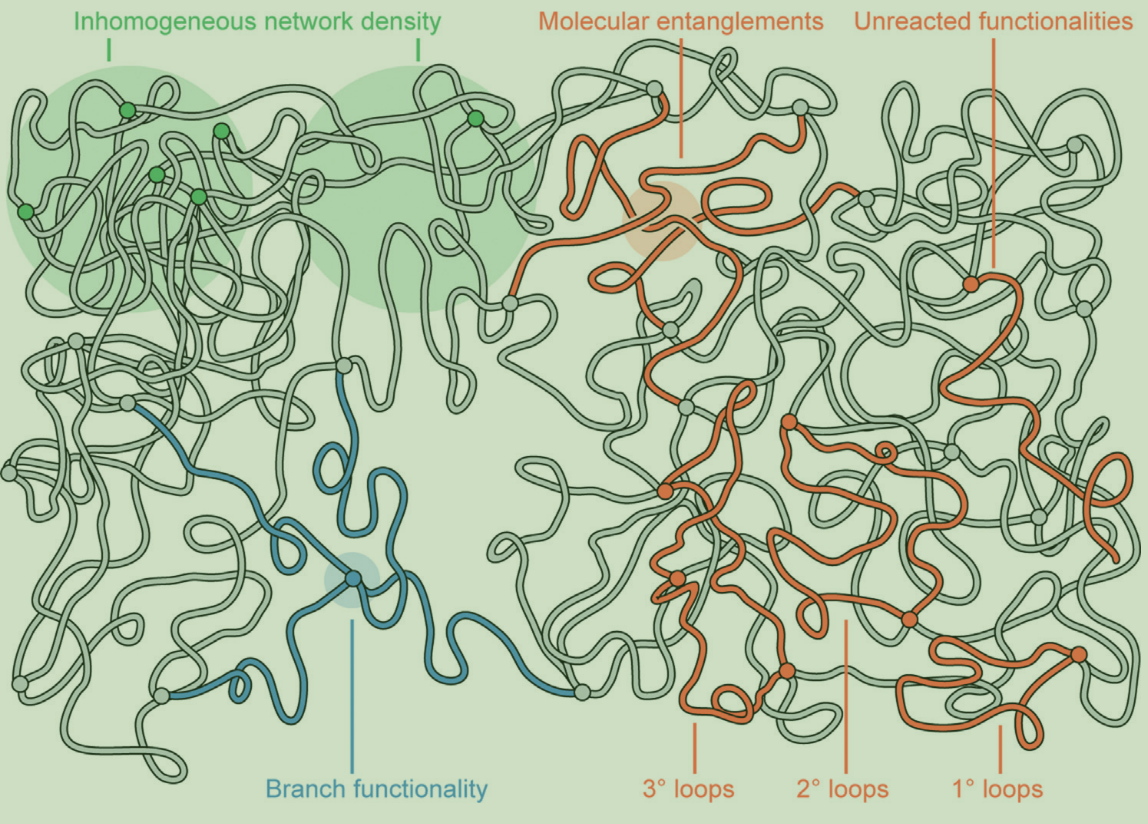
\includegraphics[width=0.8\textwidth]{figs/multilengthTopology.png}
    \caption{Multilength stuff. Scale from 10 to 100 nm shown in green, 1 to 10 nm shown in red and <1 nm shown in blue. }\label{fig:lengthScales}
\end{figure}

\paragraph{Delimit the scope} The numerical solutions allow us to explore the topology in the length scales of 5 to 100 nm ish.
We are going to describe by the general properties and stuff to the specifics of a hydrogels.
With this in mind let's introduce the idea of polymeric structures.

\subsection{Polymeric Structures}


\paragraph{Intro} From a structural standpoint, polymer networks are characterized by network ``juctions'' also known as ``crosslinks'', which consist of three or more groups departing from a core, interconnected by ``strands''.
The precise functionality of these branches is referred to as ``f''.
Strand configurations may include linear polymer chains, flexible short molecules, rigid struts/linkers, and other possible forms\citep{guPolymerNetworksPlastics2020}.

\paragraph{CrossLinking} The junctions and strands in polymer networks can be linked together via physical interactions (e.g., van der Waals interactions, hydrophobic interactions, Coulombic interactions, metalligand coordination) or covalent bonds\footnote{A deep explation is in the theoretical framework.}.
Consequently, polymer networks are conventionally classified as either ``physical'' (supramolecular) or ``chemical'' (covalent) networks.
It is important to acknowledge that this classification does not always accurately reflect material properties. 
Bond strengths and exchange rates are much more informative\footnote{To illustrate, when sufficiently strong and static physical interactions are present, physical networks can exhibit behavior analogous to that of chemical networks. 
On the other hand, the incorporation of mechanisms for covalent bond exchange can result in chemical networks that demonstrate adaptable mechanical properties regulated by external stimuli.},
because the properties of polymer networks exhibit significant variability, contingent on the composition of the junctions and strands, as well as the formation and utilization conditions.

From this point of view, virtually all polymer networks, irrespective of their colloquial designation, structural characteristics, and physical properties, can be categorically classified into one of four predominant classes: thermosets, thermoplastics, elastomers, and gels\citep{guPolymerNetworksPlastics2020}.
Given our research focus on polymer networks associated with gels, we will not delve extensively into the properties of other polymer networks. 
However, it should be noted that these networks share certain properties.

\subsection{Basic Mechanical Properties}

\paragraph{Intro} \dots are elasticity, swelling and viscoelasticity.

\paragraph{Elasticity} The physical explanation of rubber elasticity comes from the reduction in conformational entropy that occurs as a strand in a network is stretched, this process is often modeled as the unwinding of flexible, random coils. 
Once the external stretching force is removed, an elastic entropic force restores the strands to their unstretched and higher entropy state. 
Therefore, it is concluded that network strands act as entropic molecular springs\citep{guPolymerNetworksPlastics2020}. 

\paragraph{Swelling} Polymer networks constructed from strong (e.g., covalent) bonds typically do not dissolve in solvents. 
Instead, such networks absorb solvent up to an equilibrium concentration and undergo a concomitant increase in volume. 
The equilibrium degree of swelling is dictated by a balance between the free energy of polymer-solvent mixing and the free energy cost of expanding the network, which is expressed by the Flory–Rehner equation[11,133]\footnote{for isotropic swelling of an affine polymer network [Eq. (12)]:
    \begin{gather*}
        \ln(1-\phi_{\mathrm{eq}}) + \phi_{\mathrm{eq}} + \xi\phi^2_{eq} = \eta_{eff}V_1(\phi_{\mathrm{eq}}/2-\phi^{1/3}_{eq})
    \end{gather*}
}

\paragraph{Viscoelasticity} Polymeric materials exhibit both viscous and elastic characteristics upon deformation, meaning that their properties may vary with the time scale or frequency at which measurements are performed. 
To characterize this viscoelasticity with respect to tensile, compressive, or shear deformation, several types of experimental measurements are commonly applied, such as stress relaxation, creep, and oscillatory shear tests\citep{guPolymerNetworksPlastics2020}. 

\paragraph{Delimit} Now we are going to explore what is commonly refer as a hydrogel \dots to connect the elasticity, swelling and viscoelasticity to the gels.

\subsection{What is a hydrogel?}

\paragraph{}
A hydrogel is commonly describe as a material composed by a network of polymers chains that exhibits the abilitiy to swell and retain a significant fraction of water within its structure, but will not dissolve in water\citep{ahmedHydrogelPreparationCharacterization2015a,ahmedHydrogelsMicrogelsDriving2025,priyaComprehensiveReviewHydrogel2024,bustamantetorresHydrogelsClassificationAccording2021}.\footnote{the main difference with the microgels, is the size. Hydrogel is bulk, and microgelgel is particle.}
The water absorption capacity, network stability of hydrogels, and the conformation of the network with polymer chains are attributable to crosslinking mechanisms\citep{priyaComprehensiveReviewHydrogel2024,ahmedHydrogelPreparationCharacterization2015a}.
Meanwhile, the polymer chains are predominantly composed with hydrophilic functional groups and can be modified to suit a variety of applications\citep{ahmedHydrogelPreparationCharacterization2015a,priyaComprehensiveReviewHydrogel2024,bustamantetorresHydrogelsClassificationAccording2021}.

Hydrogels come in many flavors, with diverse capabilities and limitations, but in general these systems can all be described as cross-linked macromolecular networks that retain a significant amount of water. 
As much as 99\% of the weight of a hydrogel can be water, which makes these materials quite friendly to water-enriched biological environments such as the human body\citep{correaTranslationalApplicationsHydrogels2021}. 

% Hydrophilic polymers might be considered as those polymers that contain polar functional groups such as hydroxyl (-OH), carboxyl (-COOH), and amino (-NH2) groups that make them soluble or swelled by water.

While the analysis of the impact of functional groups is important, the present project prioritizes the examination of mechanisms that are more pertinent to the mechanical response. 
The crosslinking mechanisms\footnote{The hydrogels are prepared using different methods like chemical cross-linking of monomers, physical cross linking using temperature or pH changes, and blending of natural or synthetic polymers.}, in particular, are of particular interest, as they are responsible for resisting dissolution. 
This suggests that crosslinking mechanisms enable the network to undergo modification by external stimuli.

The subsequent sections will present the essential information to facilitate a comprehensive understanding of the crosslinking mechanisms, their relationship to the mechanical response, the reported mechanical response of hydrogels, and the correlation between rheology experiments and stress curves.


Here, we define dynamic hydrogels as any hydrated polymer network cross linked via reversible chemistries, which can include both covalent and noncovalent chemistries. 
Early reports of the unique rheology of dynamic networks emerged in the late 1980s with polysaccharide based networks covalently cross linked through boric esters, which  identified intriguing self healing capabilities.71 73 
However, it was only in the early 2000s that noncovalent chemistries began to be leveraged to make shear thinning supramolecular  hydrogels based on cyclodextrins,74 engineered peptides,75 and the physical interactions resulting from biopolymer  blends.76 
Although they can be prepared through diverse chemistries, dynamic hydrogels share unique rheological properties that are directly related to their translational potential as injectable systems\citep{correaTranslationalApplicationsHydrogels2021}. 

\paragraph{Overview and general problems}
In earlier technologies, harsh mechanisms for macromolecular cross-linking (e.g., toxic agents, radiation, etc.)24 28 meant that gelation needed to occur prior to introducing gels to biological systems. 
Unsurprisingly, this limited the bioengineering applications of hydrogels to superficial environments such as the surface of the eye, an open wound, or an exposed surgical bed. 
Subsequent work developed safer cross-linking mechanisms, which began a trend toward triggering gelation in situ after injection, providing a minimally invasive way of administering  hydrogels to practically any organ or tissue.29,30 
The most biocompatible iterations of these injectable in situ gelling platforms use specific cues from the body to trigger gelation:  physiological temperature,31 pH,32 or ionic strength.33 
Unlike earlier hydrogels that relied on covalent cross links, some of these hydrogels have self healing properties and possess mechanical properties akin to native tissue, capable of countering natural forces and stresses of a body in motion\citep{correaTranslationalApplicationsHydrogels2021}.

For example, significant advancements have been made to transform simple PEG based  hydrogels into responsive systems based on Boolean logic gating decisions (e.g., YES, AND, OR operations) by incorporating functional peptides and proteins into the  hydrogel network.45,49,50\citep{correaTranslationalApplicationsHydrogels2021}
Programmable biotechnologies are already leading to smart injectable materials with the potential to degrade or release drugs based on either endogenous or  exogenous triggers.51,52\citep{correaTranslationalApplicationsHydrogels2021}
As these capabilities continue to mature, multifunctional and programmable hydrogels may provide the technological foundation for platforms that can engage more effectively with the complex, multistage biological events that govern processes such as tissue regeneration and immunity.




\paragraph{Enviromental applications} 3-5 examples.

\paragraph{Medical applications} 3-5 examples.

\paragraph{Soft robots applications} 3-5 examples.

\paragraph{Smart materials} 3-5 examples.

\paragraph{Applications/Market size of the applications sectors} An overview of applications. If the previous paragraph does not convince the reader, well my last hope is that money does.

Besides, because of such a wide variety of response triggers, hydrogels can serve as sensors or actuators or can be utilized in controlled drug delivery systems, biosensors, tissue engineering scaffolds, and others [20], because of their biomimetic properties and multi functionalities [21]\citep{bustamantetorresHydrogelsClassificationAccording2021}.

In particular, biomedical applications are very popular and include cell culture [5], wound dressing and healing [2,6], drug delivery [2,7,8], tissue engineering scaffolds [9], bone repair [10], and cartilage regeneration [11]\citep{picchioniHydrogelsBasedDynamic2018}. 


The explosion of hydrogel technologies has made significant contributions in biomedical applications that impact the dayto-day lives of millions of people. 
For example, hydrogels contributions to modern life in the form of soft contact lenses, creating a new class of optically tunable soft materials and  establishing what is today a multibillion dollar industry.2 
Early studies also revealed the usefulness of engineered hydrogels for  delivering diverse drugs,3 5 establishing a field for local controlled release of bioactive compounds.6 10 
In the 1970s, surgeons recognized the utility of hydrogels for reconstructive  surgeries,11,12 and by the 1990s, hydrogels were becoming a  foundational technology for tissue regeneration.13 16 
The  history of hydrogel materials is well reviewed,17 19\footnote{Checar estas referencias} and the consistent theme has been that hydrogels continue to find new and exciting applications as the underlying technology improves.
Emerging applications for hydrogels  today include device coatings,20 environmental engineering,21  soft robotics,22 and adoptive cell therapy.23
\citep{correaTranslationalApplicationsHydrogels2021}




\section{About computer simulations}






\begin{comment}


\paragraph{Why computers and not rheometers?} Explain how in silico experiments can help to understand the relation between the network and the mechanical response.

\paragraph{Description of the Thesis} What the reader will find in each chapter and section.


\section{State of the art: Hydrogels}\label{ch1:StateArt}

\paragraph{Overview of the section.} Start from the general: Polymeric Structures.
Then go to basic properties of the polymer networks.
After that talk about gels in a broad sense.
End with applications.


\subsection{Polymeric Structures}

\subsection{Basic properties of Polymer Networks} 


\subsection{What is a hydrogel?}

\paragraph{General description of a hydrogel}


\paragraph{Examples of Hydrogels.} Give general examples of hydrogels.

\paragraph{General response.} Describe the viscoelastic response in general terms.

\paragraph{Connect properties with applications.} Transition paragraph to talk about applications.

Main review:\citep{guPolymerNetworksPlastics2020,sheikoArchitecturalCodeRubber2019}.


\subsection{Overview of mechanical properties}

The viscosity of a hydrogel is related to its injectability, elucidating the constraints that injectability places on the  viscosity of injectable biomaterials. 

For clinical applications, injectable hydrogels must be delivered through a needle or catheter to the site of injection. 

The injectability of a fluid depends on how much pressure is required to drive this process of injection over relevant time frames. 
This pressure is a function of the fluid viscosity, injection geometry, and desired flow rate. 

To elucidate these constraints on rheological properties, it is important to understand the physical process of injection. 

Injection, in its simplest form, is the flow of a fluid through a circular tube of constant diameter and length. 
Often, there is a maximum pressure that can be applied and a minimum flow rate that is desired. 
Intuitively, there is a limit to the viscosity (i.e., resistance to flow) of the materials which can be injected under a prescribed set of injection conditions and geometries. 
Therefore, it is critical to understand how viscosityand its dependence on shear rateaffects injectability, enabling researchers to use simple rheological measurements to design their materials for injectability\citep{correaTranslationalApplicationsHydrogels2021}. 

Dynamic hydrogels demonstrate rheological behavior that may comprise a combination of yielding, shear-thinning, thixotropic,  viscoelastic, and extensible behaviors.130−135 
Consequently, their characterization is nontrivial and requires a combination of rheological tests to characterize comprehensively. 
Here, we present the state-of-the-art rheological methods for measuring the viscoelastic and flow behaviors of injectable hydrogels\citep{correaTranslationalApplicationsHydrogels2021}.


\paragraph{viscoelasticity}
The viscoelasticity of a hydrogel is most often measured using dynamic mechanical analysis to measure the bulk elastic and viscous responses of a hydrogel to  an imposed oscillatory shear strain or stress.116 


\subsection{Applications}

\end{comment}

\newpage
